\newpage
\section{Iteración y solución}  

En primer lugar, se propusieron dos posibles materiales para la bandeja, Al-6061 y Ti64, cuyas propiedades se muestran en la \autoref{tab: matprops}. No obstante desde un principio la idea era hacer la bandeja de aluminio, cosa que, como se verá en las iteraciones no ha sido posible.

\begin{table}[H]
\centering
\caption{Propiedades de los materiales propuestos para la bandeja.}
\label{tab: matprops}
\begin{tabular}{c c c c c}
\toprule
\multicolumn{1}{c}{\textbf{Material}} & \multicolumn{1}{c}{$\boldsymbol{E}$ [Pa]}  & \multicolumn{1}{c}{\textbf{ $\boldsymbol{\sigma_{y}}$} [Pa]} & \multicolumn{1}{c}{$\boldsymbol{\rho}$ [kg/m$^{3}$]} & \multicolumn{1}{c}{$\boldsymbol{\nu}$ [-]} \\ \midrule
 Al 6061 &70$\cdot 10^{9}$  & 55$\cdot 10^{6}$ & 2700 & 0.33 \\
 Ti 64 & 1.138$\cdot10^{11}$ & 7$\cdot10^{8}$& 4430 &0.342 \\ \bottomrule
\end{tabular}
\end{table}

Respecto a los rigidizadores, las secciones empleadas a lo largo de las iteraciones se muestran en la \autoref{fig:Secciones}. Destacar que en el caso de los rigidizadores exteriores se han empleado secciones cuadradas exclusivamente mientras que en los interiores se ha iterado bastante modificando el tipo de sección, aunque finalmente se ha implementado también una sección rectangular hueca. 

\begin{figure}[H]  
  \begin{subfigure}[b]{0.5\linewidth}
  \centering
    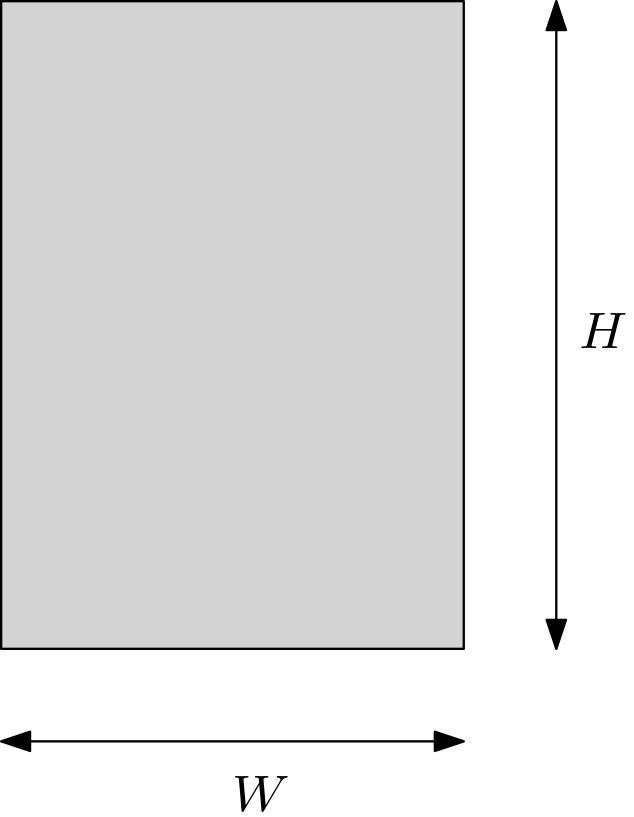
\includegraphics[scale = 0.2]{Figures/SeccExt.png} 
    \caption{Sección de los rigidizadores rectangular maciza.}
  \end{subfigure} 
  \begin{subfigure}[b]{0.5\linewidth}
  \centering
    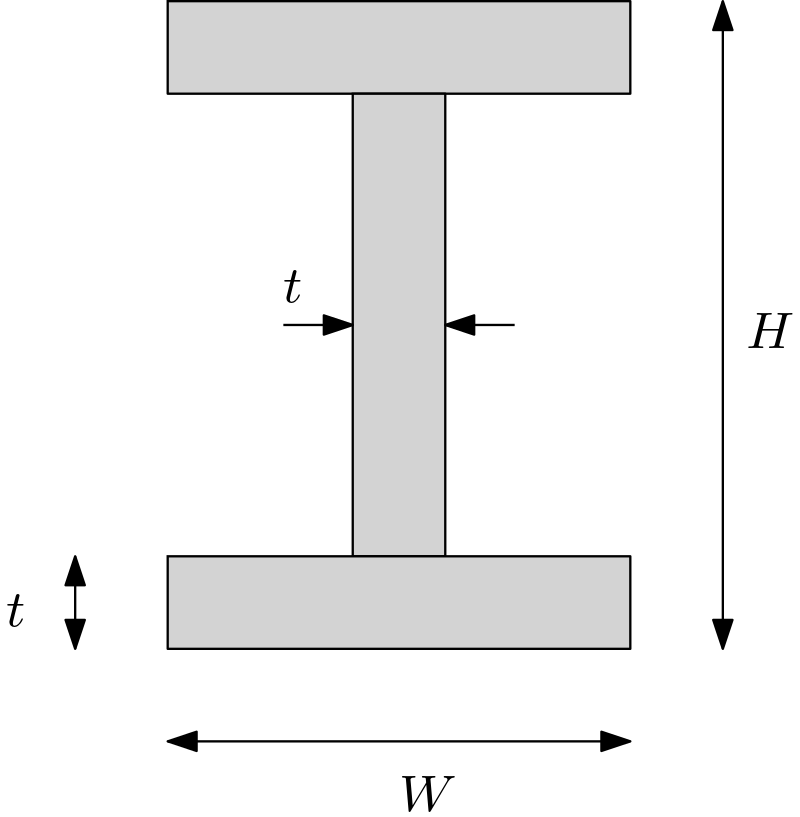
\includegraphics[scale = 0.2]{Figures/SeccI.png} 
    \caption{Sección rigidizadores  en forma de I.}
  \end{subfigure} 
  \begin{subfigure}[b]{0.5\linewidth}
  \centering
    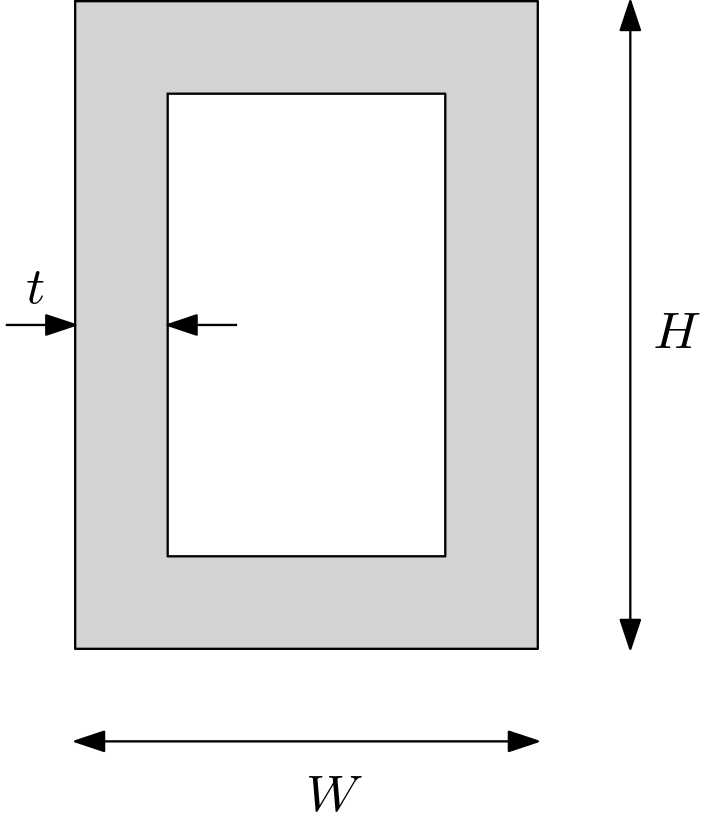
\includegraphics[scale = 0.25]{Figures/SeccCuadradoHueco.png} 
    \caption{Sección rigidizadores  rectangular hueca ($\square$).}
  \end{subfigure}
  \hfill
  \begin{subfigure}[b]{0.5\linewidth}
  \centering
    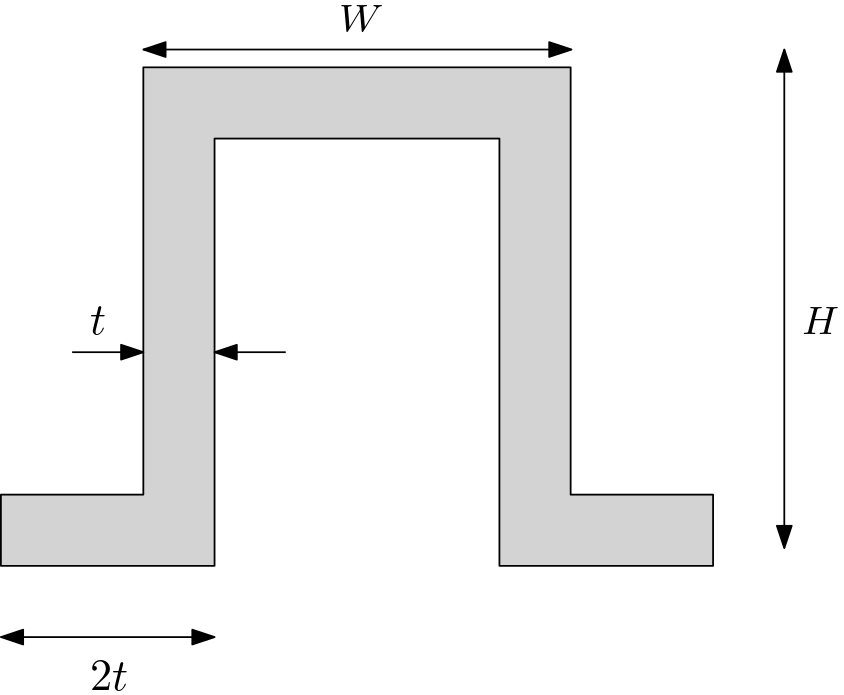
\includegraphics[scale = 0.2]{Figures/Omega.png} 
    \caption{Sección rigidizadores  en forma de $\Omega$.}
  \end{subfigure} 
 \caption{Secciones empleadas en las iteraciones.}
 \label{fig:Secciones} 
\end{figure}

El proceso iterativo se focalizó en la modificación del espesor de la bandeja y las dimensiones de los rigidizadores, tanto internos como externos, manteniendo fijo en un principio el número de rigidizadores. No obstante, tras varias iteraciones se determinó que con la disposición de rigidizadores propuesta era  inviable cumplir los requisitos estructurales, por lo que se optó por aumentar el número de rigidizadores tal y como se muestra en la \autoref{fig: rigidizadoresinternos}.

\begin{figure}[H]  
  \begin{subfigure}[b]{0.5\linewidth}
  \centering
    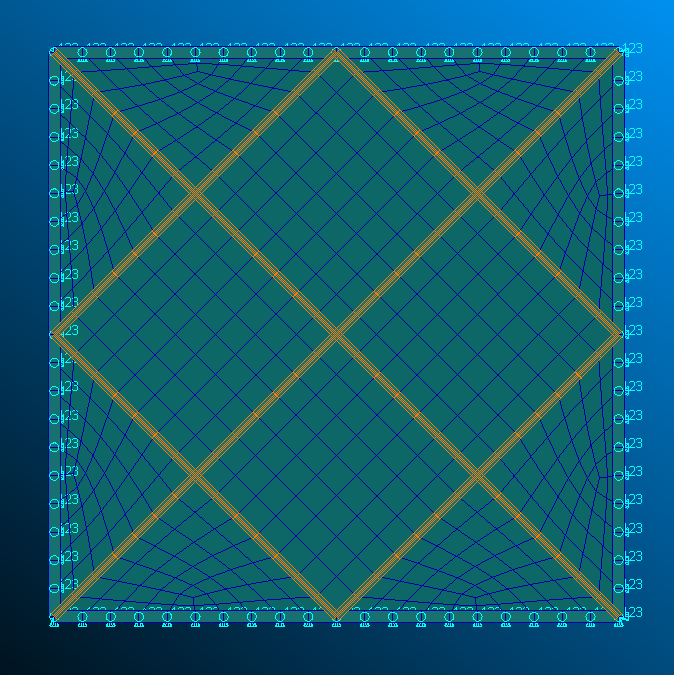
\includegraphics[scale = 0.35]{Figures/1rigpng.png} 
    \caption{Primer número de rigidizadores propuesto.}
  \end{subfigure} 
  \begin{subfigure}[b]{0.5\linewidth}
  \centering
    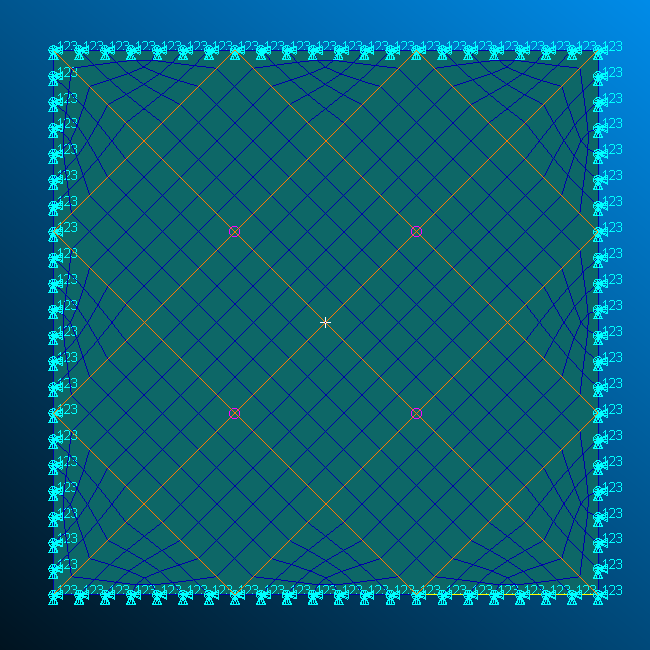
\includegraphics[scale = 0.35]{Figures/2rig.png} 
    \caption{Segundo número de rigidizadores propuesto.}
  \end{subfigure} 
  \begin{center}
  \begin{subfigure}[b]{0.5\linewidth}
  \centering
    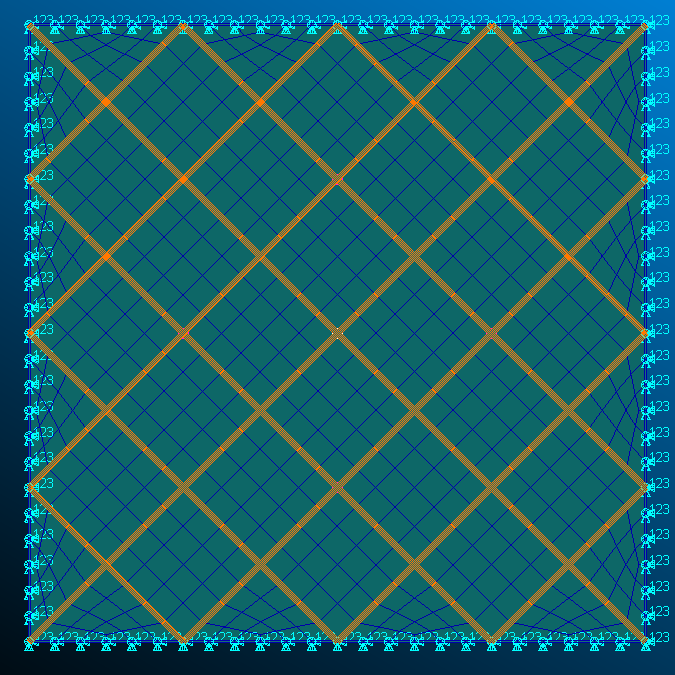
\includegraphics[scale = 0.35]{Figures/3rig.png} 
    \caption{Tercer y último número de rigidizadores propuesto.}
  \end{subfigure}
    \end{center}
 \caption{Geometrías propuestas.}
 \label{fig: rigidizadoresinternos} 
\end{figure}

Con todo esto, en la \autoref{tab:iteraciones} se muestra el proceso iterativo para esta bandeja hasta llegar al cumplimiento de ambos requisitos y la optimización de al menos uno de ellos. Además, muchas de las primeras iteraciones fueron llevadas a cabo en vano, ya que no se estaban comprobando todos los esfuerzos que se tenían que comprobar en la bandeja y sólo se estaban consultando los soportados por los elementos 2D.




\begin{table}[H]
\centering
\caption{Parametros de las iteraciones de la bandeja intermedia.}
\label{tab:iteraciones}
\resizebox{\textwidth}{!}{
\begin{tabular}{lccccccccccccc} \toprule
  \multirow{2}{*}{\textbf{It.}} & \multirow{2}{*}{$\boldsymbol{ n^{\circ}_{rig}}$} & \multirow{2}{*}{$\boldsymbol{t}$ [m]}  & \multirow{2}{*}{\textbf{Material}} & \multicolumn{2}{c}{\textbf{Rig. Exterior} [m]}  &  \multicolumn{4}{c}{\textbf{Rig. Interior} [m]}  & \multirow{2}{*}{$\boldsymbol{M}$ [kg]}  & \multirow{2}{*}{$\boldsymbol{f_o}$ [Hz]} & \multirow{2}{*}{$\boldsymbol{MOS_{y,lat}}$}   & \multirow{2}{*}{$\boldsymbol{MOS_{y,long}}$ }  \\ \cmidrule{5-6} \cmidrule{7-10}
 & & &  & $\boldsymbol{W}$ & $\boldsymbol{H}$ & \textbf{Sección} & $\boldsymbol{H}$ & $\boldsymbol{W}$ & $\boldsymbol{t} $  &   &  &  &   \\ \midrule
  
 1                     & 1                     & 3,00 $\cdot 10^{-3}$              & Al6061                & 9,50 $\cdot 10^{-3}$              & 1,30 $\cdot 10^{-2}$              & I                      & 1,50 $\cdot 10^{-2}$              & 7,00 $\cdot 10^{-3}$              & 2,00 $\cdot 10^{-3}$              & 2,58E+00              & {\cellcolor{red}}2,80 $\cdot 10^{+1}$                    & {\cellcolor{red}}-9,36 $\cdot 10^{-1}$                   & {\cellcolor{red}}-9,03 $\cdot 10^{-1}$                    \\ 
  
 2                     & 1                     & 2,00E+00              & Al6061                & 9,50 $\cdot 10^{+1}$              & 1,30 $\cdot 10^{+1}$              & I                      & 1,50 $\cdot 10^{-2}$              & 8,00 $\cdot 10^{-3}$              & 2,00 $\cdot 10^{-3}$              & 2,03E+00              & {\cellcolor{red}}2,49 $\cdot 10^{+1}$                    & -                                            & -                                             \\ 
  
 3                     & 1                     & 4,00 $\cdot 10^{-3}$              & Al6061                & 1,50 $\cdot 10^{-2}$              & 1,50 $\cdot 10^{-2}$              & I                      & 1,50 $\cdot 10^{-2}$              & 7,00 $\cdot 10^{-3}$              & 3,00 $\cdot 10^{-3}$              & 3,13E+00              & {\cellcolor{red}}3,39 $\cdot 10^{+1}$                    & -                                            & -                                             \\ 
  
 4                     & 1                     & 3,00 $\cdot 10^{-3}$              & Ti64                  & 9,50 $\cdot 10^{-3}$              & 1,30 $\cdot 10^{-2}$              & I                      & 1,50 $\cdot 10^{-2}$              & 7,00 $\cdot 10^{-3}$              & 2,00 $\cdot 10^{-3}$              & 3,37E+00              & {\cellcolor{red}}3,30 $\cdot 10^{+1}$                    & -                                            & -                                             \\ 
  
 5                     & 1                     & 4,00 $\cdot 10^{-3}$              & Ti64                  & 9,50 $\cdot 10^{-3}$              & 1,30 $\cdot 10^{-2}$              & I                      & 1,50 $\cdot 10^{-2}$              & 7,00 $\cdot 10^{-3}$              & 2,00 $\cdot 10^{-3}$              & 3,67E+00              & {\cellcolor{red}}3,54 $\cdot 10^{+1}$                    & -                                            & -                                             \\ 
  
 6                     & 1                     & 4,00 $\cdot 10^{-3}$              & Ti64                  & 9,50 $\cdot 10^{-3}$              & 1,30 $\cdot 10^{-2}$              & I                      & 1,50 $\cdot 10^{-2}$              & 7,00 $\cdot 10^{-3}$              & 2,00 $\cdot 10^{-3}$              & 3,57E+00              & {\cellcolor{red}}4,05 $\cdot 10^{+1}$                    & -                                            & -                                             \\ 
  
 7                     & 1                     & 4,00 $\cdot 10^{-3}$              & Ti64                  & 1,00 $\cdot 10^{-2}$              & 1,50 $\cdot 10^{-2}$              & I                      & 1,50 $\cdot 10^{-2}$              & 7,00 $\cdot 10^{-3}$              & 2,00 $\cdot 10^{-3}$              & 3,27E+00              & {\cellcolor{red}}4,10 $\cdot 10^{+1}$                    & -                                            & -                                             \\ 
  
 8                     & 1                     & 4,00 $\cdot 10^{-3}$              & Ti64                  & 1,00 $\cdot 10^{-2}$              & 1,50 $\cdot 10^{-2}$              & I                      & 1,50 $\cdot 10^{-2}$              & 1,50 $\cdot 10^{-2}$              & 3,00 $\cdot 10^{-3}$              & 3,97E+00              & {\cellcolor{red}}5,52 $\cdot 10^{+1}$                    & -                                            & -                                             \\ 
  
 9                     & 1                     & 4,00 $\cdot 10^{-3}$              & Ti64                  & 1,50 $\cdot 10^{-2}$              & 1,50 $\cdot 10^{-2}$              &  \Omega  & 1,50 $\cdot 10^{-2}$              & 7,00 $\cdot 10^{-3}$              & 3,00 $\cdot 10^{-3}$              & 4,67E+00              & {\cellcolor{red}}5,56 $\cdot 10^{+1}$                    & -                                            & -                                             \\ 
  
 10                    & 1                     & 5,00 $\cdot 10^{-3}$              & Ti64                  & 1,50 $\cdot 10^{-2}$              & 1,50 $\cdot 10^{-2}$              &  \Omega  & 1,50 $\cdot 10^{-2}$              & 7,00 $\cdot 10^{-3}$              & 3,00 $\cdot 10^{-3}$              & 5,59E+00              & {\cellcolor{red}}6,13 $\cdot 10^{+1}$                    & -                                            & -                                             \\ 
  
 11                    & 1                     & 5,00 $\cdot 10^{-3}$              & Ti64                  & 1,50 $\cdot 10^{-2}$              & 1,50 $\cdot 10^{-2}$              &  \square & 1,50 $\cdot 10^{-2}$              & 1,50 $\cdot 10^{-2}$              & 3,00 $\cdot 10^{-3}$              & 2,58E+00              & {\cellcolor{red}}6,86 $\cdot 10^{+1}$                    & -                                            & -                                             \\ 
  
 12                    & 1                     & 5,00 $\cdot 10^{-3}$              & Ti64                  & 1,50 $\cdot 10^{-2}$              & 1,50 $\cdot 10^{-2}$              &  \square & 2,00 $\cdot 10^{-2}$              & 1,00 $\cdot 10^{-2}$              & 3,00 $\cdot 10^{-3}$              & 2,03E+00              & {\cellcolor{red}}5,70 $\cdot 10^{+1}$                    & -                                            & -                                             \\ 
  
 13                    & 1                     & 5,00 $\cdot 10^{-3}$              & Ti64                  & 1,50 $\cdot 10^{-2}$              & 1,50 $\cdot 10^{-2}$              &  \square & 2,00 $\cdot 10^{-2}$              & 1,00 $\cdot 10^{-2}$              & 3,00 $\cdot 10^{-3}$              & 3,13E+00              & {\cellcolor{red}}7,81 $\cdot 10^{+1}$                    & -                                            & -                                             \\ 
  
 14                    & 1                     & 5,00 $\cdot 10^{-3}$              & Ti64                  & 1,50 $\cdot 10^{-2}$              & 1,50 $\cdot 10^{-2}$              &  \square & 2,00 $\cdot 10^{-2}$              & 1,00 $\cdot 10^{-2}$              & 4,00 $\cdot 10^{-3}$              & 3,37E+00              & {\cellcolor{red}}8,14 $\cdot 10^{+1}$                    & -                                            & -                                             \\ 
  
 15                    & 1                     & 5,00 $\cdot 10^{-3}$              & Ti64                  & 1,50 $\cdot 10^{-2}$              & 1,50 $\cdot 10^{-2}$              &  \square & 2,00 $\cdot 10^{-2}$              & 1,00 $\cdot 10^{-2}$              & 4,00 $\cdot 10^{-3}$              & 3,67E+00              & {\cellcolor{red}}7,90 $\cdot 10^{+1}$                    & -                                            & -                                             \\ 
  
 16                    & 1                     & 5,00 $\cdot 10^{-3}$              & Ti64                  & 1,50 $\cdot 10^{-2}$              & 1,50 $\cdot 10^{-2}$              &  \square & 2,00 $\cdot 10^{-2}$              & 1,00 $\cdot 10^{-2}$              & 4,00 $\cdot 10^{-3}$              & 3,57E+00              & {\cellcolor{red}}8,14 $\cdot 10^{+1}$                    & -                                            & -                                             \\ 
  
 17                    & 1                     & 5,00 $\cdot 10^{-3}$              & Ti64                  & 1,00 $\cdot 10^{-2}$              & 1,50 $\cdot 10^{-2}$              &  \square & 2,25 $\cdot 10^{-2}$              & 1,00 $\cdot 10^{-2}$              & 4,00 $\cdot 10^{-3}$              & 3,27E+00              & {\cellcolor{red}}8,72 $\cdot 10^{+1}$                    & -                                            & -                                             \\ 
  
 18                    & 1                     & 5,00 $\cdot 10^{-3}$              & Ti64                  & 1,00 $\cdot 10^{-2}$              & 1,50 $\cdot 10^{-2}$              &  \square & 2,50 $\cdot 10^{-2}$              & 1,00 $\cdot 10^{-2}$              & 4,00 $\cdot 10^{-3}$              & 5,59E+00              & {\cellcolor{red}}9,52 $\cdot 10^{+1}$                    & -                                            & -                                             \\ 
  
 19                    & 1                     & 5,00 $\cdot 10^{-3}$              & Ti64                  & 1,00 $\cdot 10^{-2}$              & 1,50 $\cdot 10^{-2}$              &  \square & 2,60 $\cdot 10^{-2}$              & 1,00 $\cdot 10^{-2}$              & 4,00 $\cdot 10^{-3}$              & 2,58E+00              & {\cellcolor{red}}9,84 $\cdot 10^{+1}$                    & -                                            & -                                             \\ 
  
 20                    & 2                     & 2,00 $\cdot 10^{-3}$              & Al6061                & 1,00 $\cdot 10^{-2}$              & 1,30 $\cdot 10^{-2}$              &  \square & 1,20 $\cdot 10^{-2}$              & 5,00 $\cdot 10^{-3}$              & 2,00 $\cdot 10^{-3}$              & 1,63E+00              & {\cellcolor{red}}7,34 $\cdot 10^{+1}$                    & -                                            & -                                             \\ 
  
 21                    & 2                     & 3,00 $\cdot 10^{-3}$              & Al6061                & 1,00 $\cdot 10^{-2}$              & 1,30 $\cdot 10^{-2}$              &  \square & 1,30 $\cdot 10^{-2}$              & 5,00 $\cdot 10^{-3}$              & 2,00 $\cdot 10^{-3}$              & 1,64E+00              & {\cellcolor{yellow}}1,34 $\cdot 10^{+2}$                 & {\cellcolor{red}}-9,87 $\cdot 10^{-1}$                   & {\cellcolor{red}}-9,68 $\cdot 10^{-1}$                    \\ 
  
 22                    & 2                     & 2,00 $\cdot 10^{-3}$              & Al6061                & 5,00 $\cdot 10^{-3}$              & 1,30 $\cdot 10^{-2}$              &  \square & 1,40 $\cdot 10^{-2}$              & 5,00 $\cdot 10^{-3}$              & 2,00 $\cdot 10^{-3}$              & 1,14E+00              & {\cellcolor{red}}7,34 $\cdot 10^{+1}$                    & -                                            & {\cellcolor{red}}-9,86 $\cdot 10^{-1}$                    \\ 
  
 23                    & 2                     & 2,50 $\cdot 10^{-3}$              & Al6061                & 5,00 $\cdot 10^{-3}$              & 1,30 $\cdot 10^{-2}$              &  \square & 1,40 $\cdot 10^{-2}$              & 5,00 $\cdot 10^{-3}$              & 2,00 $\cdot 10^{-3}$              & 1,36E+00              & {\cellcolor[rgb]{0.439,0.678,0.278}}1,02 $\cdot 10^{+2}$ & {\cellcolor{red}}-9,91 $\cdot 10^{-1}$                   & -                                             \\ 
  
 24                    & 2                     & 3,00 $\cdot 10^{-3}$              & Al6061                & 5,00 $\cdot 10^{-3}$              & 1,30 $\cdot 10^{-2}$              &  \square & 1,00 $\cdot 10^{-2}$              & 1,00 $\cdot 10^{-2}$              & 2,00 $\cdot 10^{-3}$              & 1,36E+00              & {\cellcolor[rgb]{0.439,0.678,0.278}}1,02 $\cdot 10^{+2}$ & {\cellcolor{red}}-9,91 $\cdot 10^{-1}$                   & -                                             \\ 
  
 25                    & 2                     & 4,00 $\cdot 10^{-3}$              & Al6061                & 1,00 $\cdot 10^{-2}$              & 1,50 $\cdot 10^{-2}$              &  \square & 1,50 $\cdot 10^{-2}$              & 1,00 $\cdot 10^{-2}$              & 2,00 $\cdot 10^{-3}$              & 3,91E+00              & {\cellcolor{red}}6,70 $\cdot 10^{+1}$                    & {\cellcolor{red}}-8,19 $\cdot 10^{-1}$                   & -                                             \\ 
  
 26                    & 2                     & 5,00 $\cdot 10^{-3}$              & Al6061                & 1,00 $\cdot 10^{-2}$              & 1,50 $\cdot 10^{-2}$              &  \square & 1,50 $\cdot 10^{-2}$              & 1,00 $\cdot 10^{-2}$              & 2,00 $\cdot 10^{-3}$              & 4,00E+00              & {\cellcolor{red}}7,04 $\cdot 10^{+1}$                    & -                                            & -                                             \\ 
  
 27                    & 2                     & 5,00 $\cdot 10^{-3}$              & Al6061                & 1,00 $\cdot 10^{-2}$              & 1,50 $\cdot 10^{-2}$              &  \square & 1,50 $\cdot 10^{-2}$              & 1,00 $\cdot 10^{-2}$              & 2,00 $\cdot 10^{-3}$              & 4,00E+00              & {\cellcolor{red}}7,04 $\cdot 10^{+1}$                    & -                                            & -                                             \\ 
  
 28                    & 2                     & 6,00 $\cdot 10^{-3}$              & Al6061                & 1,00 $\cdot 10^{-2}$              & 1,50 $\cdot 10^{-2}$              &  \square & 1,50 $\cdot 10^{-2}$              & 1,00 $\cdot 10^{-2}$              & 2,00 $\cdot 10^{-3}$              & 4,00E+00              & {\cellcolor{red}}7,58 $\cdot 10^{+1}$                    & -                                            & -                                             \\ 
  
 29                    & 3                     & 3,00 $\cdot 10^{-3}$              & Al6061                & 1,00 $\cdot 10^{-2}$              & 1,50 $\cdot 10^{-2}$              &  \square & 1,50 $\cdot 10^{-2}$              & 1,00 $\cdot 10^{-2}$              & 2,00 $\cdot 10^{-3}$              & 4,00E+00              & {\cellcolor{red}}8,96 $\cdot 10^{+1}$                    & -                                            & -                                             \\ 
  
 30                    & 3                     & 3,50 $\cdot 10^{-3}$              & Al6061                & 1,00 $\cdot 10^{-2}$              & 1,50 $\cdot 10^{-2}$              &  \square & 1,50 $\cdot 10^{-2}$              & 1,00 $\cdot 10^{-2}$              & 2,00 $\cdot 10^{-3}$              & 4,00E+00              & {\cellcolor{red}}9,33 $\cdot 10^{+1}$                    & -                                            & -                                             \\ 
  
 31                    & 3                     & 3,50 $\cdot 10^{-3}$              & Al6061                & 1,10 $\cdot 10^{-2}$              & 1,50 $\cdot 10^{-2}$              &  \square & 1,60 $\cdot 10^{-2}$              & 1,00 $\cdot 10^{-2}$              & 2,00 $\cdot 10^{-3}$              & 4,00E+00              & {\cellcolor{red}}9,76 $\cdot 10^{+1}$                    & -                                            & -                                             \\ 
  
 32                    & 3                     & 3,50 $\cdot 10^{-3}$              & Al6061                & 1,10 $\cdot 10^{-2}$              & 1,60 $\cdot 10^{-2}$              &  \square & 1,60 $\cdot 10^{-2}$              & 1,00 $\cdot 10^{-2}$              & 2,00 $\cdot 10^{-3}$              & 4,36E+00              & {\cellcolor[rgb]{0.439,0.678,0.278}}1,04 $\cdot 10^{+2}$ & {\cellcolor{red}}-5,21 $\cdot 10^{-1}$                   & -                                             \\ 
  
 33                    & 3                     & 3,50 $\cdot 10^{-3}$              & Al6061                & 1,60 $\cdot 10^{-2}$              & 1,60 $\cdot 10^{-2}$              &  \square & 1,60 $\cdot 10^{-2}$              & 1,00 $\cdot 10^{-2}$              & 2,00 $\cdot 10^{-3}$              & 4,81E+00              & {\cellcolor[rgb]{0.439,0.678,0.278}}1,11 $\cdot 10^{+2}$ & {\cellcolor{red}}-5,21 $\cdot 10^{-1}$                   & -                                             \\ 
  
 34                    & 3                     & 4,00 $\cdot 10^{-3}$              & Al6061                & 1,00 $\cdot 10^{-2}$              & 1,60 $\cdot 10^{-2}$              &  \square & 1,60 $\cdot 10^{-2}$              & 1,00 $\cdot 10^{-2}$              & 2,00 $\cdot 10^{-3}$              & 4,41E+00              & {\cellcolor[rgb]{0.439,0.678,0.278}}1,03 $\cdot 10^{+2}$ & {\cellcolor{red}}-4,26 $\cdot 10^{-1}$                   & -                                             \\ 
  
 35                    & 3                     & 5,00 $\cdot 10^{-3}$              & Al6061                & 1,00 $\cdot 10^{-2}$              & 1,60 $\cdot 10^{-2}$              &  \square & 1,60 $\cdot 10^{-2}$              & 1,00 $\cdot 10^{-2}$              & 2,00 $\cdot 10^{-3}$              & 4,96E+00              & {\cellcolor[rgb]{0.439,0.678,0.278}}1,12 $\cdot 10^{+2}$ & {\cellcolor{red}}-3,45 $\cdot 10^{-1}$                   & {\cellcolor[rgb]{0.439,0.678,0.278}}3,10 $\cdot 10^{-2}$  \\ 
  
 36                    & 3                     & 5,00 $\cdot 10^{-3}$              & Al6061                & 1,00 $\cdot 10^{-2}$              & 1,60 $\cdot 10^{-2}$              &  \square & 1,60 $\cdot 10^{-2}$              & 1,00 $\cdot 10^{-2}$              & 2,00 $\cdot 10^{-3}$              & 5,41E+00              & {\cellcolor{yellow}}1,36 $\cdot 10^{+2}$                 & {\cellcolor{red}}-1,28 $\cdot 10^{-1}$                   & -                                             \\ 
  
 37                    & 3                     & 5,00 $\cdot 10^{-3}$              & Al6061                & 1,00 $\cdot 10^{-2}$              & 2,00 $\cdot 10^{-2}$              &  \square & 2,00 $\cdot 10^{-2}$              & 1,00 $\cdot 10^{-2}$              & 2,00 $\cdot 10^{-3}$              & 5,41E+00              & {\cellcolor{yellow}}1,36 $\cdot 10^{+2}$                 & {\cellcolor{red}}-1,28 $\cdot 10^{-1}$                   & -                                             \\ 
  
 38                    & 3                     & 5,00 $\cdot 10^{-3}$              & Al6061                & 1,50 $\cdot 10^{-2}$              & 2,50 $\cdot 10^{-2}$              &  \square & 2,50 $\cdot 10^{-2}$              & 1,50 $\cdot 10^{-2}$              & 2,00 $\cdot 10^{-3}$              & 6,52E+00              & {\cellcolor{yellow}}1,78 $\cdot 10^{+2}$                 & {\cellcolor{red}}-1,26 $\cdot 10^{-1}$                   & -                                             \\ 
  
 39                    & 3                     & 1,00 $\cdot 10^{-3}$              & Al6061                & 1,00 $\cdot 10^{-2}$              & 2,00 $\cdot 10^{-2}$              &  \square & 2,00 $\cdot 10^{-2}$              & 1,00 $\cdot 10^{-2}$              & 2,00 $\cdot 10^{-3}$              & 4,24E+00              & {\cellcolor{yellow}}1,42 $\cdot 10^{+2}$                 & {\cellcolor{red}}-5,53 $\cdot 10^{-1}$                   & -                                             \\ 
  
 40                    & 3                     & 2,00 $\cdot 10^{-3}$              & Ti64                  & 1,00 $\cdot 10^{-2}$              & 2,00 $\cdot 10^{-2}$              &  \square & 2,00 $\cdot 10^{-2}$              & 1,00 $\cdot 10^{-2}$              & 2,00 $\cdot 10^{-3}$              & 2,72E+00              & {\cellcolor[rgb]{0.439,0.678,0.278}}1,03 $\cdot 10^{+2}$ & {\cellcolor[rgb]{0.439,0.678,0.278}}1,63 $\cdot 10^{-1}$ & {\cellcolor[rgb]{0.439,0.678,0.278}}1,25E+00  \\
  
  \bottomrule
\end{tabular}
}
\end{table}

Finalmente, tras un total de \textbf{40 iteraciones} se llegó a la solución con los parámetros mostrados en la \autoref{tab:paramsfinales}.

\begin{table}[H]
\centering
\caption{Parámetros de diseño de solución encontrada.}
\label{tab:paramsfinales}
\begin{tabular}{cccccccccccc} \toprule
\multirow{2}{*}{$\boldsymbol{n^{\circ}_{rig}}$} &\multirow{2}{*}{\textbf{Espesor} [m]} &\multirow{2}{*}{\textbf{Material} } & & \multicolumn{2}{c}{\textbf{Rig. Exterior} [m]} & & \multicolumn{4}{c}{\textbf{Rig. Interior} [m]} \\ \cmidrule{4-5} \cmidrule{7-10}
                      &                        & & $\boldsymbol{H}$             & $\boldsymbol{W }$           &   & \textbf{Sección}     & $\boldsymbol{H}$     & $\boldsymbol{W }$    & $\boldsymbol{t}$   \\ \midrule
   3                    &  $2\cdot 10^{-3}$   & Ti64   &         &     2$\cdot 10^{-3}$        &      1$\cdot 10^{-3}$       &  &  $\square$   &   2$\cdot 10^{-2}$  & 1$\cdot 10^{-2}$   & 2$\cdot 10^{-3}$    \\ \bottomrule
\end{tabular}
\end{table}

Con estos parámetros se ha conseguido optimizar la masa a la vez que se optimiza el criterio del margen de seguridad más critico, tal y como se muestra en la \autoref{tab:propsol}.

\begin{table}[H]
\centering
\caption{Propiedades de la bandeja final.}
\label{tab:propsol}
\begin{tabular}{cccc} \toprule
\multicolumn{1}{c}{\textbf{Masa} [kg]} & \textbf{1ª f. propia} [Hz] & $\boldsymbol{MOS_{y,\text{\textbf{long}}}}$ & $\boldsymbol{MOS_{y,\text{\textbf{lat}}}}$ \\ \midrule
  2.72   & 103.12   & 1.25  & 1.63$\cdot 10^{-1}$    \\ \bottomrule
\end{tabular}
\end{table}

Cabe destacar que las mayores tensiones se han visto los ensayos laterales sobre los elementos placa cercanos a los laterales de la bandeja. En la \autoref{fig: finalfinal} se muestran el primer modo propio de la bandeja (\autoref{fig:modopropio}) y la distribución de tensiones en estos casos mencionados (\autoref{fig:longitudiz} longitudinal y \autoref{fig:laterallllllllll} lateral) .

\begin{figure}[H]  
  \begin{subfigure}[b]{0.5\linewidth}
   \centering
    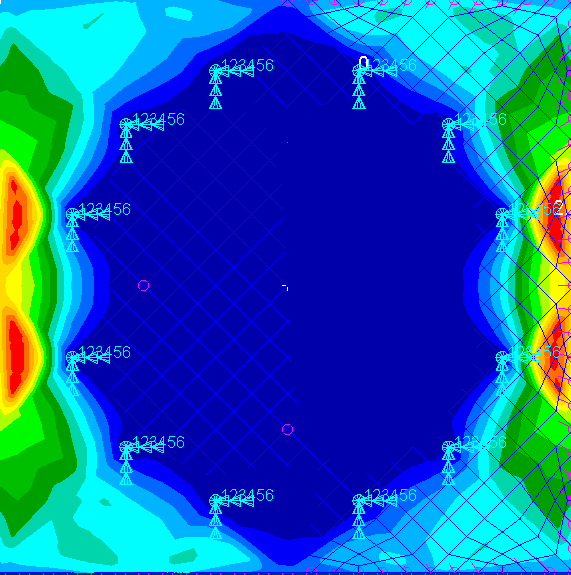
\includegraphics[width=\linewidth]{Figures/FrecProp.png} 
    \caption{Modo propio de respiración.}
    \label{fig:modopropio}
  \end{subfigure} 
  \begin{subfigure}[b]{0.5\linewidth}
   \centering
    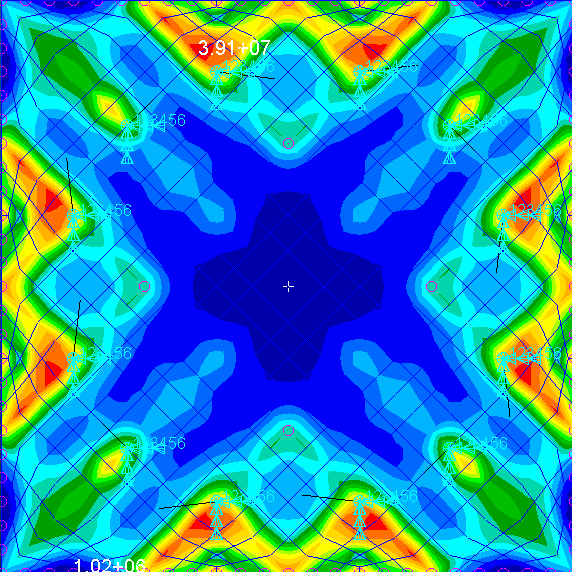
\includegraphics[width=\linewidth]{Figures/StaticZ.png} 
    \caption{Análisis estático longitudinal.}
    \label{fig:longitudiz}
  \end{subfigure} 
  \begin{center}
  \begin{subfigure}[b]{0.5\linewidth}
   \centering
    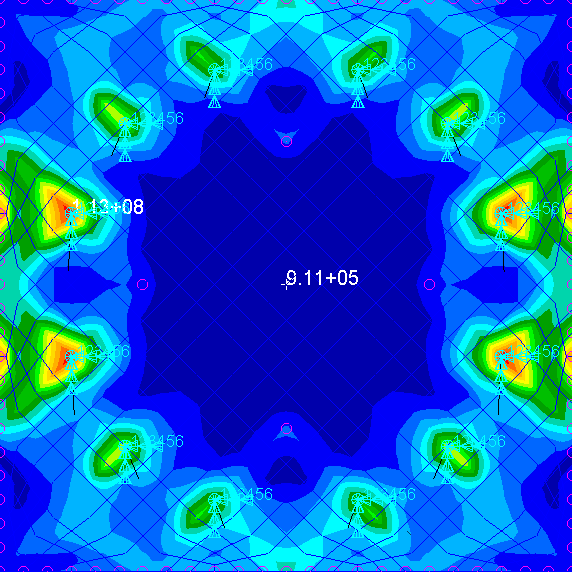
\includegraphics[width=\linewidth]{Figures/StaticXY.png} 
    \caption{Análisis estático lateral.}
    \label{fig:laterallllllllll}
  \end{subfigure}
    \end{center}
 \caption{Primer modo propio y distribución de tensiones en la bandeja.}
 \label{fig: finalfinal} 
\end{figure}